% IEEEtran journal layout from the user-supplied Hyper-IIoT source.
% `letterpaper` is the supported spelling of its `lettersize` option.
\documentclass[letterpaper,journal]{IEEEtran}
\usepackage{amsmath,amssymb,amsfonts,amsthm}
\usepackage{graphicx,array,booktabs,tabularx,multirow,textcomp}
\usepackage{xcolor,indentfirst,cite,xurl}
\usepackage{algorithm,algorithmicx,algpseudocode}
\usepackage[hidelinks]{hyperref}
\usepackage{orcidlink}
\usepackage{placeins}
\setlength{\textfloatsep}{10pt plus 2pt minus 2pt}
\setlength{\dbltextfloatsep}{10pt plus 2pt minus 2pt}
\hyphenation{op-tical net-works semi-conduc-tor}
\newtheorem{proposition}{Proposition}
\newtheorem{definition}{Definition}
\newcommand{\T}{\mathcal T}
\newcommand{\Lang}{\mathcal L}
\title{SPR-IoT: Static MQTT Policy Repair under Topic-Language and Deployment Constraints}
\author{Dun~Li\,\orcidlink{0000-0002-1986-7144},
Zibin~Zheng\,\orcidlink{0000-0001-7872-7718},~\IEEEmembership{Fellow,~IEEE},
Hongzhi~Li\textsuperscript{*}\,\orcidlink{0000-0002-5883-3780},
Noel~Crespi\,\orcidlink{0000-0003-2962-192X},
and~Wei~Liang\,\orcidlink{0000-0002-5074-1363},~\IEEEmembership{Senior~Member,~IEEE}%
\thanks{Dun Li is with the Department of Industrial Engineering, Tsinghua University, Beijing 100084, China (e-mail: \href{mailto:lidun.2023@tsinghua.org.cn}{lidun.2023@tsinghua.org.cn}).}%
\thanks{Zibin Zheng is with the School of Software Engineering, Sun Yat-sen University, Zhuhai 510275, China (e-mail: \href{mailto:zhzibin@mail.sysu.edu.cn}{zhzibin@mail.sysu.edu.cn}).}%
\thanks{Hongzhi Li is with the College of Big Data and Artificial Intelligence, Chizhou University, Chizhou 247100, China (e-mail: \href{mailto:pickpickup@sohu.com}{pickpickup@sohu.com}). \textsuperscript{*}Corresponding author: Hongzhi Li.}%
\thanks{Noel Crespi is with Samovar, Telecom SudParis, Institut Polytechnique de Paris, 91120 Palaiseau, France (e-mail: \href{mailto:noel.crespi@mines-telecom.fr}{noel.crespi@mines-telecom.fr}).}%
\thanks{Wei Liang is with the School of Computer / School of Software, University of South China, Hengyang 421001, China (e-mail: \href{mailto:wliang@usc.edu.cn}{wliang@usc.edu.cn}).}}
\hypersetup{pdfauthor={Dun Li; Zibin Zheng; Hongzhi Li; Noel Crespi; Wei Liang}}
\date{}
\begin{document}
\markboth{SPR-IoT: Static MQTT Policy Repair}{SPR-IoT: Static MQTT Policy Repair}
\maketitle


% BEGIN_SECTION front
\begin{abstract}
Finite-topic repairs of MQTT access policies can leave forbidden descendants accessible or block legitimate new branches. SPR-IoT represents required and forbidden communication as topic languages and jointly models subscription authorization, filter matching and receive authorization. It searches bounded policy-edit combinations while enforcing Mosquitto Dynamic Security deployment constraints. Repair cost is minimized within a declared finite edit grammar; unsupported inputs and inconsistent requirements are reported separately. An independent interpreter and actual Broker delivery checks validate exported policies. On 36 controlled specifications, historical exact and quotient backends each complete 34 repairs versus 30 for a strictly improving greedy reference. A separate matched rerun shows that allowing one neutral bridge also reaches 34, closing this template-specific gap. Quotienting removes no candidates and shows no stable efficiency benefit. All 127 historical Broker probes agree with concrete predictions. Public AWS scenarios are evaluated separately under researcher-supplemented finite requirements. These results support static repair within fixed-subscription, single-role and printable-ASCII boundaries; natural-error and unrestricted-client generalization remain unestablished.
\end{abstract}
\begin{IEEEkeywords}
MQTT, Internet of Things, access control, policy repair, topic languages, formal verification.
\end{IEEEkeywords}

\section{Introduction}
\IEEEPARstart{I}{oT} topic namespaces expand with new devices, measurements and tenants. Monitoring clients may require future public topics while remaining excluded from private descendants. MQTT delivery combines subscription authorization, filter matching and receive authorization~\cite{mqtt311,mosquitto_dynsec}. Exact-topic Denies can miss forbidden descendants; finite whitelists can block legitimate new branches (Figure~\ref{fig:problem_overview}). Both requirements therefore concern topic languages, not just currently enumerated topics.

\begin{figure}[!t]\centering
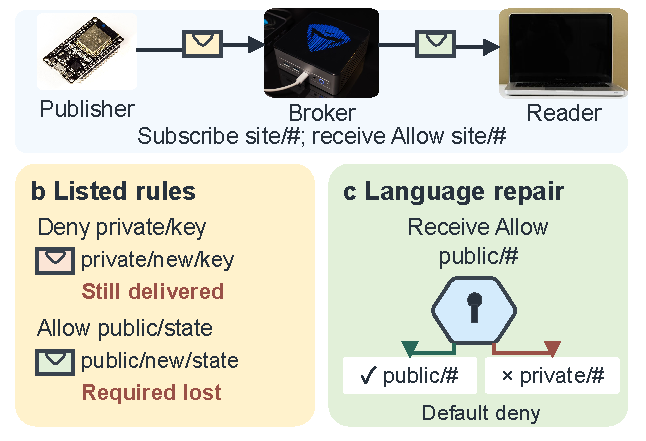
\includegraphics[width=\linewidth]{figures/intro_problem.pdf}
\caption{Topic-language repair: exact Deny misses private descendants, while exact whitelist loses public descendants; receive-Allow narrowing preserves/excludes the respective languages. Lower panels omit \texttt{site/}; authorized publisher assumed. Illustrative photos: Ubahnverleih (CC0), Kaboompics/Matheus Bertelli (Pexels). Experiments are single-host.}\label{fig:problem_overview}
\end{figure}

Repair poses two coupled challenges: preserving required communication while excluding forbidden languages, and ensuring that the resulting edit combination can be deployed. Deny-all and retaining every Allow fail opposite obligations. Moreover, language-equivalent rules can occupy different deployment keys; replacing one without its conflict context may discard an otherwise deployable repair.

SPR-IoT combines language checking, deployment-valid bounded search and independent execution checks. Direct exact enumeration is the standard backend; contextual quotienting is optional. Evaluation separates controlled MQTT structures, finite public AWS scenarios and real Broker behavior, examining both communication obligations and complete repair cost.

\subsection{Related Work}
\paragraph{Communication and policy verification}
P-Verifier analyzes effective cloud-IoT communication, including receive authorization~\cite{pverifier,pverifier_code}; IOT:POKER checks information-flow reachability~\cite{iotpoker}; MQTTactic verifies Broker logic~\cite{mqttactic}. Semantic analyses also address SELinux flows~\cite{selinux_flow}, administrative reachability~\cite{admincbac}, ABAC hierarchies~\cite{semantic_abac} and explicit-Deny conversion~\cite{deny_conversion}. SPR-IoT connects delivery languages to deployable edits and Broker execution.

\paragraph{Policy repair and refinement}
Quantitative Policy Repair uses symbolic analysis and model counting to reduce permissiveness to a specified bound while retaining designated must-allow requests~\cite{quantitative_repair}. IAM-PolicyRefiner retains observed permissions during local refinement~\cite{iam_refiner}; CloudFix validates language-model-generated IAM repairs~\cite{cloudfix}. Policy generation~\cite{sok_nl} and permission-check identification~\cite{pcfinder} address requirements and enforcement. Our obligations are supplied topic languages, not automatically inferred from Allows or history.

\paragraph{IoT authorization and execution}
Blockchain supports trustworthy digital-twin exchange~\cite{li_dt_survey}, ABE authorization~\cite{dt_abe} and information-centric services~\cite{icn_survey}. DPS-IIoT uses zero-knowledge-proof-inspired, CP-ABE and blockchain authorization~\cite{li_dps}; Hyper-IIoT uses smart-contract-assisted ABAC~\cite{li_hyper}. Other mechanisms address bilateral protection~\cite{pdcs}, cross-domain authorization~\cite{scpa}, interoperability~\cite{crossplatform}, accountable tokens~\cite{tbac} and auditable automata~\cite{event_audit}. SPR-IoT repairs the static scope supplied to these mechanisms.

Zero-trust usage control~\cite{ztaiot}, token attenuation~\cite{stateful_auth} and revocation~\cite{evoke} concern lifecycle behavior. FECAC~\cite{fecac}, scalable IoT authorization~\cite{scalable_iot} and Linux ABAC~\cite{linux_abac} address execution cost; we distinguish repair, deployment and communication costs.

\subsection{Our Contributions}
\begin{itemize}
\item Explicit required/forbidden delivery languages with fixed-subscription sufficiency conditions.
\item Deployment-valid finite edit combinations and sufficient contextual replacement conditions.
\item Independent concrete interpretation and Mosquitto validation, separating controlled and public-derived scenarios.
\end{itemize}

\subsection{Organization}
Section~II defines policies, requirements and subscription scope. Section~III presents checking, deployment-valid repair and validation. Section~IV evaluates communication, rule interactions and computation/deployment costs. Section~V concludes and outlines future work.
% END_SECTION front


% BEGIN_SECTION problem
\section{Problem Definition}
\subsection{Supported Snapshot and Topic Languages}
Fix reader $p$, its username/client ID and one directly assigned role, without additional role/group grants. Policies use explicit default deny, one subscription-ACL kind and unique priorities per event. The highest-priority match decides; keys follow Mosquitto 2.1.2~\cite{mosquitto_dynsec,mosquitto_roles212}.

Let $\T$ contain nonempty printable-ASCII topics, at most 65,535 bytes, excluding literal \texttt{+}/\texttt{\#}. Each character occupies one byte. Empty levels and leading/trailing/repeated separators are supported. In $\Lang(f)\subseteq\T$, \texttt{+} matches one level, final \texttt{\#} all remaining levels; root wildcards exclude \texttt{\$}-prefixed topics. ASCII restricts the implementation, not MQTT~\cite{mqtt311}.

Supported events are literal or restricted-pattern subscription authorization and message receive authorization. Literal approval of \texttt{a/\#} differs from matching its language. The checker rejects shared subscriptions, identity variables, multi-role composition, priority ties, Unicode, retained messages and session lifecycles.

\subsection{Effective Delivery and Hard Requirements}
Let $F$ be a finite catalogue of proposed subscription filters. Define
\begin{equation}
 A(P,F)=\{f\in F:\operatorname{SUB}_P(p,f)=\mathsf{allow}\}.
\end{equation}
For a topic $t$, $\operatorname{RECV}_P(p,t)$ is the decision of the highest-priority matching receive ACL, or deny by default. Write $V_P=\{t\in\T:\operatorname{RECV}_P(p,t)=\mathsf{allow}\}$. Under an authorized external-publisher premise, effective delivery is
\begin{equation}\label{eq:delivery}
 D(P,F)=V_P\cap\bigcup_{f\in A(P,F)}\Lang(f).
\end{equation}
Authentication, identity binding and publisher authorization are fixed preconditions; connection or publisher failure cannot count as a repair.

Required communication $R$ and forbidden communication $B$ are explicit unions of topic-filter languages. A complete repair satisfies
\begin{equation}\label{eq:req}
 R\subseteq D(P,F),\qquad D(P,F)\cap B=\varnothing.
\end{equation}
Availability preserves a compliant route to each required topic; unspecified requests remain unconstrained. $R\cap B\ne\varnothing$ means conflict. Consistent but inexpressible requirements mean declared-space infeasibility; timeout and unsupported input are separate.

\subsection{Subscription Sufficiency and Threat Scope}
Equation~\eqref{eq:delivery} covers every $t\in\T$ but only $f\in F$. For all plain filters $H_P$ authorized by the deployed policy, extending this conclusion requires
\begin{equation}\label{eq:closure}
 \bigcup_{h\in H_P}\Lang(h)\ \subseteq
 \bigcup_{f\in A(P,F)}\Lang(f).
\end{equation}
Otherwise an authorized filter outside $F$ can reach forbidden topics: grant \texttt{a/\#} with $F=\{\texttt{a/public}\}$ does not cover subscriptions to \texttt{a/private/\#}.

Literal grants within $F$, or a maximal approved prefix filter, establish this condition. Repairs add no subscription grants. Shared subscriptions were not globally disabled: their raw request strings remain outside this plain-interface guarantee.

The attacker chooses topics and routes within this static interface; unrestricted raw MQTT clients are not covered. Identity compromise, additional policy attachments, dynamic revocation and unmodeled protocol paths are excluded.

\subsection{Separate AWS Interpretation}
The offline AWS adapter treats resource \texttt{*}/\texttt{?} as string wildcards, unlike MQTT \texttt{+}/\texttt{\#}; \texttt{topicfilter}/\texttt{topic} authorize different events~\cite{aws_policy}. Its condition-free finite subset uses explicit-deny precedence. Variables, complex conditions, AWS-to-Mosquitto translation and full multi-policy composition~\cite{aws_engine} are unsupported.
% END_SECTION problem


% BEGIN_SECTION design
\section{System Model and Design}
\subsection{System Architecture}
Figure~\ref{fig:architecture} maps inputs to repairs/classified failures. E checks communication/deployment; Q optionally preprocesses the same space. Counterexamples diagnose existing options. Independent interpretation and Broker execution validate exports.

\begin{figure*}[!t]\centering
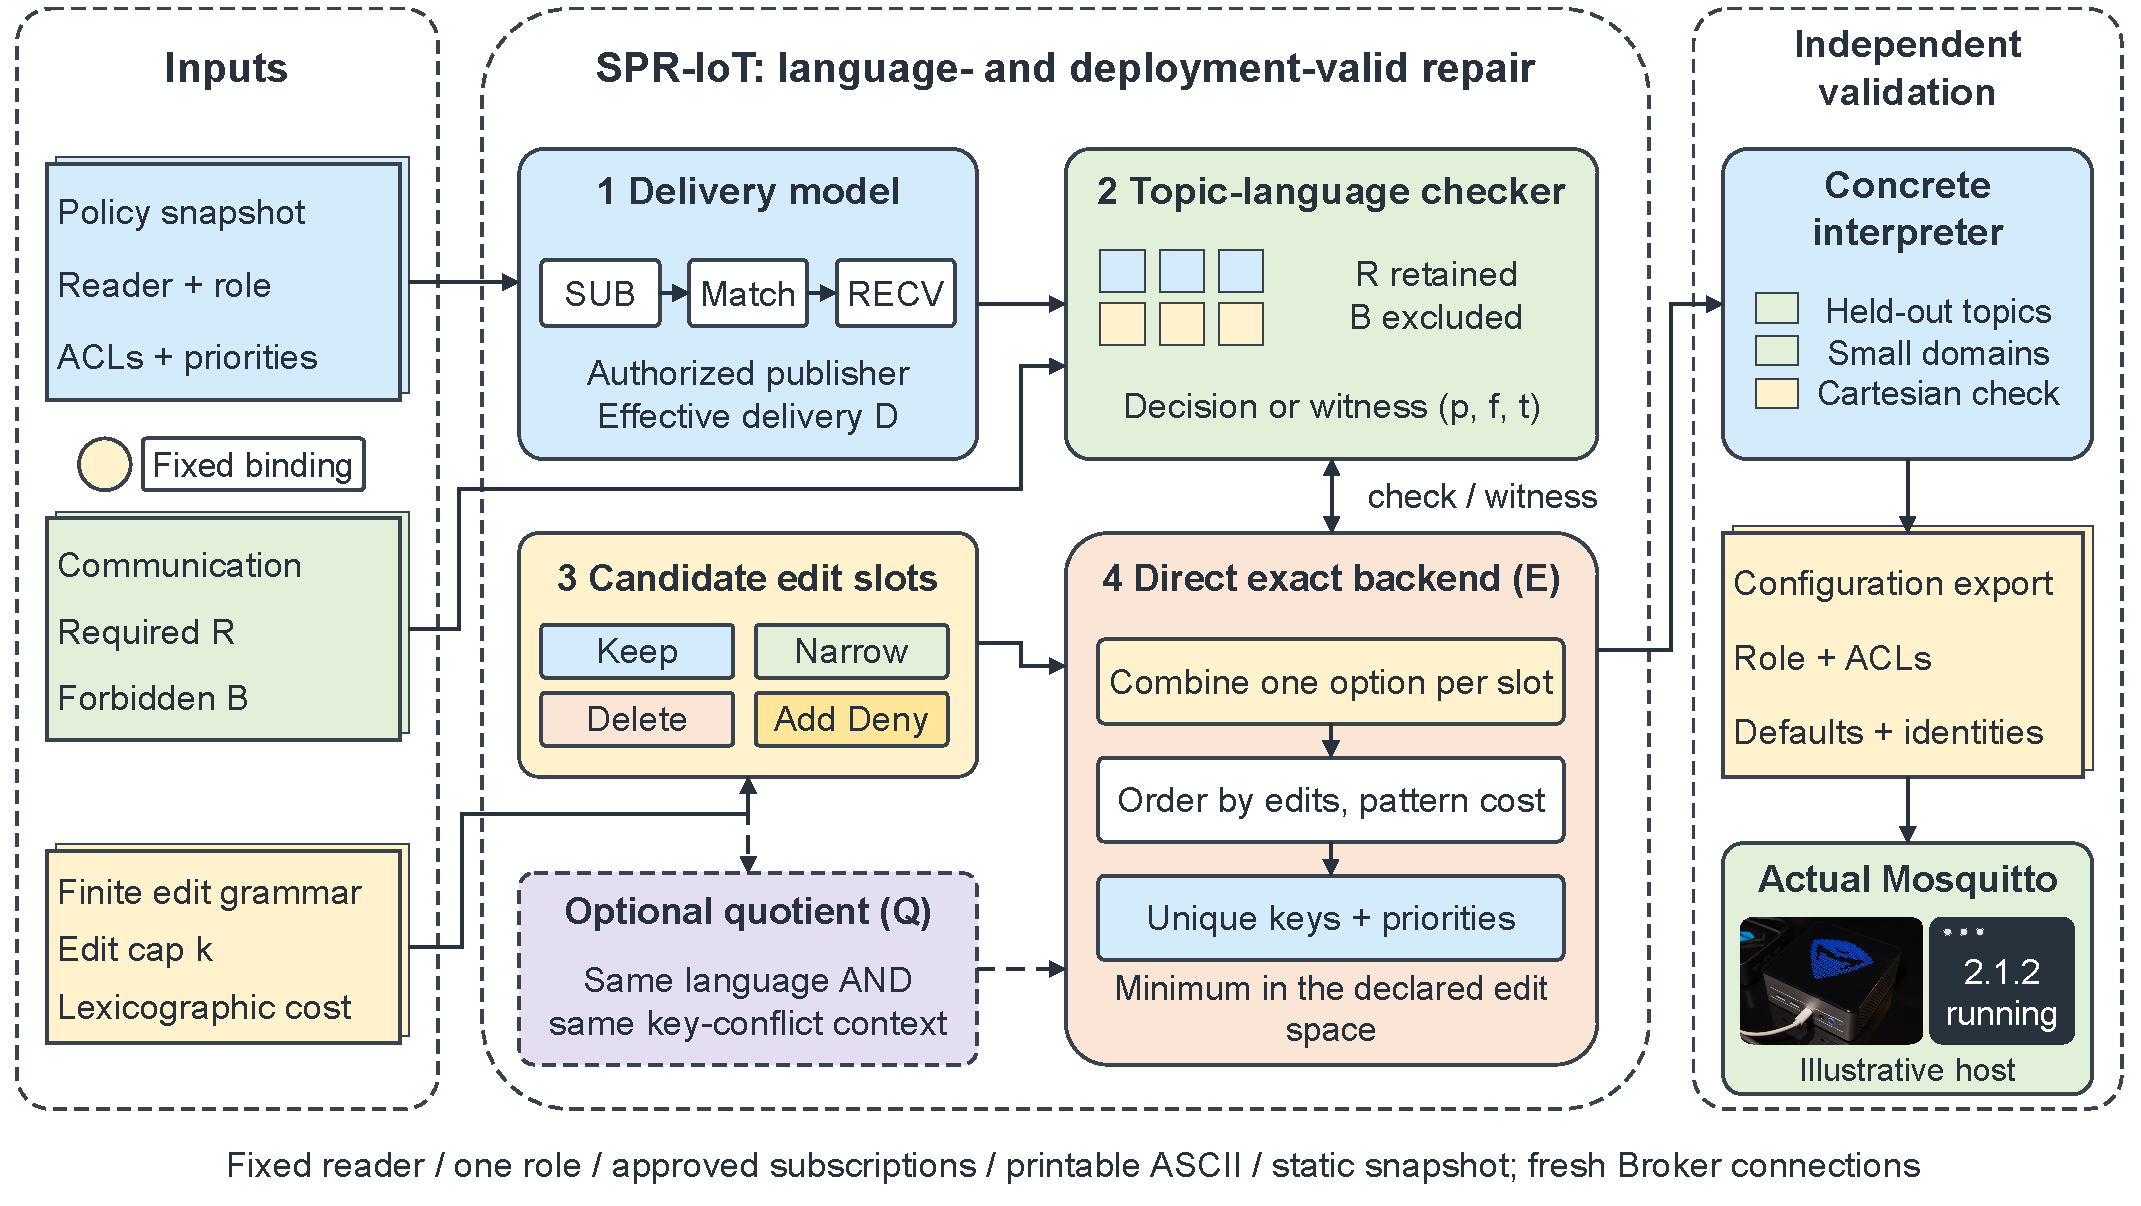
\includegraphics[width=\textwidth]{figures/system_architecture.pdf}
\caption{SPR-IoT processing and validation. Dashed paths denote optional contextual quotienting. Broker observations are finite; the host photo is illustrative (Matheus Bertelli/Pexels), and status text restates the startup log.}\label{fig:architecture}
\end{figure*}

\subsection{Topic-Language Checking and Counterexamples}
The validated checker searches forbidden and missing witnesses:
\[
 W_{\rm forbidden}=D(P,F)\cap B,\qquad
 W_{\rm missing}=R\setminus D(P,F).
\]
The check passes iff both sets are empty. Forbidden witnesses identify a topic, authorized filter and matching rules; missing witnesses identify required topics without delivery. SUBSCRIBE success alone is insufficient.

A filter-state product partitions levels into literal, empty, ordinary nonliteral and root-dollar classes. Shortest legal representatives and separator-weighted lengths enforce nonempty topics and the byte limit; transitions preserve membership and delivery.

Each concrete witness maps to an abstract path of no greater byte length; accepted paths reconstruct legal witnesses. Independent bounded tests cover empty levels, root-dollar behavior and byte limits, without constituting a machine-checked or full-MQTT proof.

\subsection{Deployment-Valid Combination Repair}
Original slots permit keep/delete and receive-Allow narrowing. Seeds use declared requests/requirements and fixed single-level/subtree generalizations, with symbolic containment checks. Additional slots permit forbidden-pattern receive denies above existing priorities. Identities, roles, defaults and original priorities are fixed.

Let $U_i$ be the ordered choices for immutable slot $i$, with index set $\mathcal J_i=\{0,\ldots,|U_i|-1\}$ and zero denoting its unedited state. The operation cost and cap-bounded assignment space are
\begin{equation}\label{eq:assignments}\begin{aligned}
 c_{\rm operations}(a)&=\sum_{i=1}^{m}\mathbf{1}[a_i\ne0],\\
 \mathcal A_k&=\left\{a\in\prod_{i=1}^{m}\mathcal J_i:c_{\rm operations}(a)\le k\right\}.
\end{aligned}\end{equation}
Deletion, replacement and addition each cost one operation; remove/add deployment replacement is one logical edit. Changed originals and additions are separate counts. Pattern cost sums edited levels/wildcards; minimize lexicographically:
\begin{equation}\begin{aligned}
 &\min\bigl(c_{\rm operations},c_{\rm pattern}\bigr)\\
 &\text{subject to~\eqref{eq:req} and deployment validity.}
\end{aligned}\end{equation}
Optimality and infeasibility concern only this grammar and cap; timeout proves neither.

Let $P_a$ materialize assignment $a$. Deployment validity $\operatorname{Valid}(P_a)$ preserves supported rule kinds, role, identity and defaults, and requires, for distinct materialized rules $r,s$,
\begin{equation}\label{eq:deployment}\begin{aligned}
 \operatorname{key}(r)&\ne\operatorname{key}(s),\\
 \operatorname{event}(r)=\operatorname{event}(s)
 &\Rightarrow\operatorname{priority}(r)\ne\operatorname{priority}(s).
\end{aligned}\end{equation}
Keys use $(\operatorname{event},\operatorname{topic})$, with literal topic strings. One choice per slot prevents repeated/conflicting edits; materialization is order-independent.

Algorithm~\ref{alg:repair} rejects invalid deployments before language checking. It returns the first feasible assignment in fixed cost order; declared-space infeasibility requires exhaustion.

\begin{algorithm}[!t]
\caption{Bounded deployment-valid combination repair}\label{alg:repair}
\begin{algorithmic}[1]
\Require Snapshot $P$, approved filters $F$, languages $R,B$, cap $k$
\Ensure Minimum-cost repair or classified outcome
\State Validate the snapshot; reject unsupported input
\If{$R\cap B\ne\varnothing$}
 \State \Return requirement conflict
\EndIf
\State Generate ordered slot choices $U_1,\ldots,U_m$
\State Optionally quotient under Section~III-D's conditions
\State Enumerate $\mathcal A_k$; sort by cost and canonical indices
\For{each assignment $a$ in this order}
 \State Materialize $P_a$
 \If{$\operatorname{Valid}(P_a)$}
  \If{$R\subseteq D(P_a,F)$ and $D(P_a,F)\cap B=\varnothing$}
   \State Independently audit; \Return $P_a$ and edits
  \EndIf
 \EndIf
\EndFor
\State \Return infeasible in the declared space
\Statex An external deadline returns timeout at any stage.
\end{algorithmic}
\end{algorithm}

Generating and sorting all cap-bounded assignments still incurs time and memory; the complete budget includes preprocessing and output.

\subsection{Context-Preserving Candidate Quotient}
\paragraph{Deployment-key counterexample}
A regression grants literal subscription \texttt{\#}, receive-Allow \texttt{\#} (priority 2) and receive-Deny \texttt{/\#} (1); it requires \texttt{/\#} and forbids \texttt{a/\#}, \texttt{b/\#}. Over nonempty topics, \texttt{/\#} and \texttt{/+/\#} are language-equivalent. Narrowing the Allow to the former duplicates the Deny's key; the latter is valid. Earlier language-only pruning retained the cheaper invalid option, a defect in our representation, not the Broker.

Exact/Cartesian and contextual quotient both return cost $(1,5)$ at caps one/two. The old quotient incorrectly prunes all cap-one repairs and returns $(2,3)$ at cap two. Costs are (operations, pattern complexity).


For option $r$ in slot $i$, let $U_j$ be the full option set of slot $j$. Define its full-space key-conflict footprint
\begin{equation}\begin{aligned}
 K_i(r)=\{(j,u): {}&j\ne i,\ u\in U_j,\\
 &\operatorname{key}(r)=\operatorname{key}(u)\}.
\end{aligned}\end{equation}
Q requires equal event/effect/priority, receive languages (or decisions on $F$) and full unpruned conflict footprints, with nonincreasing additive cost~\cite{moito}. Absence merges only with itself; language/signature equality alone is insufficient.

\begin{proposition}[Sufficient contextual replacement conditions]
For the fixed-slot model above, suppose replacement preserves event decisions and priority, preserves every cross-slot deployment-key conflict, and does not increase local additive cost or edit count. Replacing an option by its retained representative preserves validity and delivery in every other-slot context, and does not increase the total objective or violate the edit cap. If each discarded option has such a representative, the quotient preserves the optimum in the declared space.
\end{proposition}
\begin{proof}
Equal key-conflict footprints preserve whether any selected option in another slot aliases the candidate key. Equal priority preserves priority-tie validity; remaining grammar conditions are unchanged. Equal event decisions under the same ordering preserve receive decisions and subscription decisions on $F$, hence preserve $D(P,F)$. The local cost and edit-count inequalities are additive across slots. Mapping each full-space feasible assignment to representatives thus gives a no-more-expensive feasible quotient assignment. The quotient is also a subset of the full space, yielding equality of optimal costs.
\end{proof}



\subsection{Configuration Export and Independent Validation}
Independent interpretation checks held-out topics/small domains; Cartesian enumeration checks caps, priorities, keys and optima. AWS checking uses dynamic programming, not optimizer regexes. A new literal-only export preflight rejects inconsistent bindings, extra roles/groups, permissive defaults, priority/key conflicts and grants outside $F$. It checks configuration, not raw requests.

Fresh Mosquitto configurations retain identities, roles, defaults and ACLs. Message IDs, acknowledgments, receipts, forwarding logs and before/after observer controls establish finite execution consistency.
% END_SECTION design


% BEGIN_SECTION evaluation
\section{Performance Evaluation and Analysis}\label{sec:eval}
\subsection{Experimental Environment and Configuration}
Table~\ref{tab:design} separates evaluation strata and units. Safety, availability and joint completion are distinct; costs use their stated populations~\cite{iam_metrics}.

Historical runs use Python 3.14.7/Mosquitto 2.1.2, Windows 11, 32 logical processors and loopback; CPU model/RAM capacity were unrecorded; load was not isolated. Connections are fresh. Five-second child budgets cover generation through output; parent time adds startup, validation, I/O and cleanup. RSS is peak working set. Caps: reference/semantic/demand two; pressure three unless scanned.

\begin{table*}[!t]\centering\small
\caption{Evaluation strata and units. Timing reuses specifications; messages are nested within runs. Delivery F/G follows the fixed representative schedule.}\label{tab:design}
\begin{tabularx}{\textwidth}{@{}p{29mm}p{31mm}p{30mm}X@{}}\toprule
Stratum & Specifications / scope & Methods & Repetition unit\\\midrule
Reference & 6 & O,D,W,F,G,E,Q & One run per specification/method\\
Topic semantics & 12 & F,G,E,Q & One run; four separately varied factors\\
Pressure & 36 / 4 templates & G,E,Q & One run; 15 initial-language classes\\
Nested demand & 3 levels & G,E,Q & One run per level/method\\
Search conditions & 13 & G,E,Q & One run; separate factor families\\
Paired timing & 4 existing reps. & E,Q & 5 full-run pairs each; no new tasks\\
Cap/overlap grid & 4 cells & E,Q & One run per cell/method\\
Finite AWS & 20 scenarios & E,Q & 11 overgrant, 5 safe, 2 deficit, 2 injected\\
\bottomrule\end{tabularx}\end{table*}

\begin{figure*}[!t]\centering
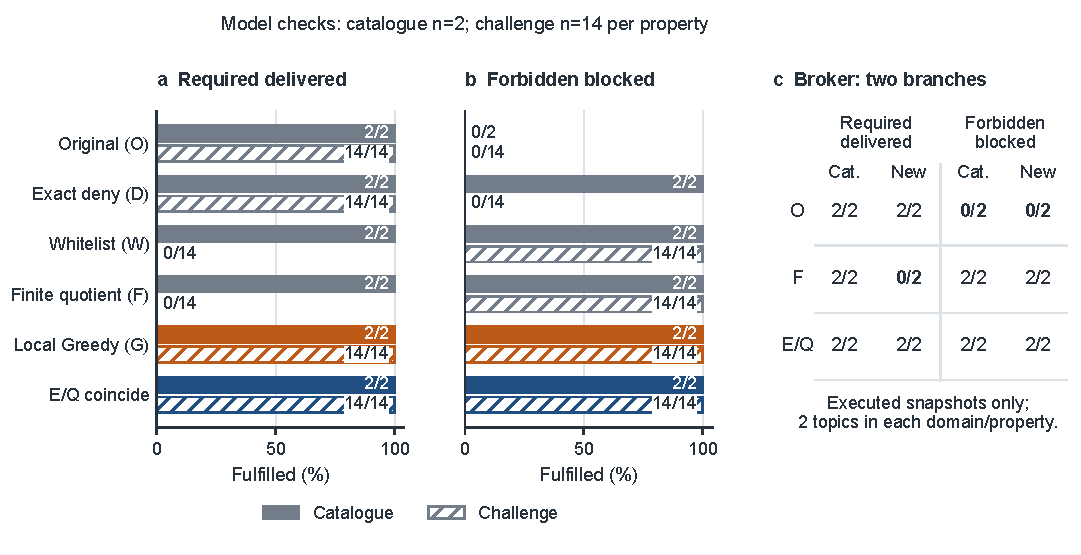
\includegraphics[width=\textwidth]{figures/01_communication.pdf}
\caption{Communication preservation and exclusion. Model catalogue/challenge counts use $n=2/14$ per property; executed Broker cells use $n=2$ (Cat./New). Domains remain separate; E/Q combine only equal counts. O is unrepaired. Finite observations retain the model scope.}\label{fig:communication}
\end{figure*}

\begin{figure*}[!t]\centering
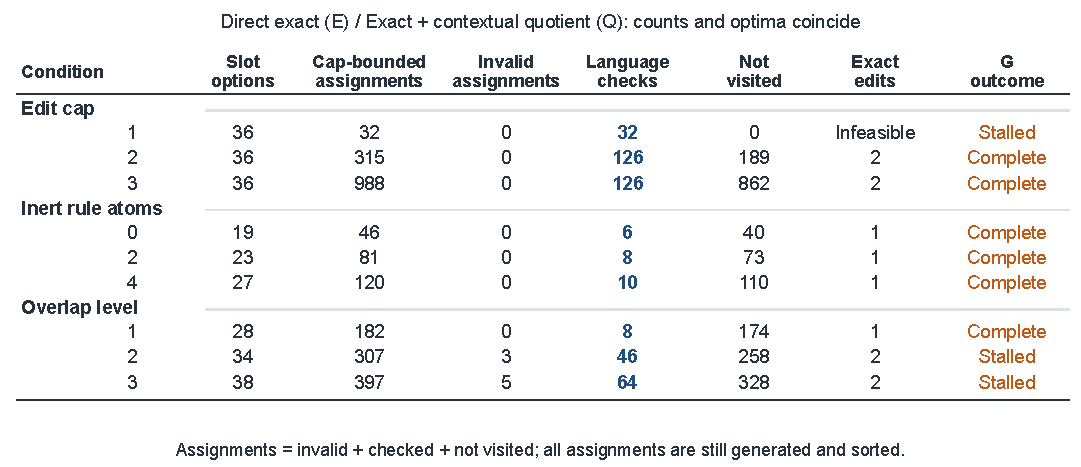
\includegraphics[width=\textwidth]{figures/02_mechanisms.pdf}
\caption{Three separate search families; E/Q counts and optima coincide. Generated/sorted assignments partition into rejected, checked and unvisited. Cap one is infeasible. G's score counter is a different unit.}\label{fig:mechanisms}
\end{figure*}

G/E/Q share edits, deployment validity, cost and budget. For pattern unions $R=\bigcup_{u=1}^{n_R}R_u$, $B=\bigcup_{v=1}^{n_B}B_v$, G counts violations:
\begin{equation}\label{eq:greedy-score}\begin{aligned}
 \nu(P)={}&\sum_{u=1}^{n_R}\mathbf{1}[R_u\not\subseteq D(P,F)]\\
 &+\sum_{v=1}^{n_B}\mathbf{1}[D(P,F)\cap B_v\ne\varnothing].
\end{aligned}\end{equation}
G edits unchanged slots only, requiring $\nu(P')<\nu(P)$; ties use cost/canonical indices. It stops at completion, cap or no improvement; stall is not infeasibility. O is original; D/W/F are exact Deny/finite whitelist/finite quotient, without open guarantees. The CloudFix repair pipeline was not reproduced and is not a measured baseline. The non-optimal baseline $G_{N1}$ permits one bridge after a G stall: $\nu(P_1)=\nu(P)$ and $\nu(P_2)<\nu(P)$, with both policies valid, different untouched slots and sufficient remaining cap; endpoint ties follow G.

The first five strata total seventy specifications. Four templates $\times$ scales 1--3 $\times$ three language settings yield 36 pressure specifications/fifteen initial-language classes. Development-inspected conditions are not independent sources or blind confirmation. Totals: 286 controlled (forty timing), eight grid and forty AWS runs.

P-Verifier yields 541 unique whole documents from 834 JSON files and, separately, 547 unique Statement wrappers from 969 occurrences. Keys sort; arrays retain order. CloudFix has 276 unique/282 valid documents, 22 IoT-related. Researcher-supplemented B requirements give eleven overgrants (six P-Verifier policies, one template), five safe/two mixed-undergrant diagnoses. CloudFix 252/67 add only safe/deficit cases; two C tasks inject official-example errors. Allows are not business truth; natural-error generalization is unestablished.

Of 74 controlled/grid configurations, 71 grant literals within $F$; three include maximal prefix filters. All forty Broker snapshots use literal grants within $F$, one reader role, no groups and explicit deny defaults.

Twenty offline pairs give fifteen completions (branches/overlap/strong demand, five each) and five double-timeouts. Four Broker representatives yield 10/16 executed delivery slots; three conflicts/two timeouts/one G stall lack policies. Four unselected combinations are outside the schedule. Overhead executes 30/40 slots; five conflicts/five timeouts leave 10/20 complete pairs (branches/overlap, five each). Missing differences are never zero-filled.



\subsection{Topic-Language Preservation and Repair Effectiveness}
Figure~\ref{fig:communication} compares catalogue/challenge behavior. D misses forbidden descendants; W/F lose required challenges. G/E/Q satisfy both obligations; E/Q agree per condition. Symbolic checks separately establish language properties.

Executed Broker snapshots confirm O's forbidden delivery, F's required-challenge loss and E/Q's preservation/exclusion. D/W were not deployed.



Twelve dependent conditions give F safety 12/12, availability 3/12; G/E/Q satisfy both on 12/12. Separate factors are coverage (2/6, 4/6, 6/6), depth (4--6), required shape (exact/one-level/subtree) and challenges (2, 4, 6). Flat outcomes imply neither factor interactions nor infinite-space coverage.

Reference G/E/Q complete 4/6, including one safe control; the rest conflict or lack reachable business. Safety/availability: O 1/6, 5/6; W 5/6, 0/6; D 1/6, 4/6; F 4/6, 1/6. Success requires both.

Finite AWS E/Q complete 11/11 supplemented overgrants and 2/2 injected cases, each at one operation. Five safe controls are unchanged; two deficits are infeasible under non-expanding edits. Enumerated Receive Deny suffices here, without open-AWS, difficult multi-edit or natural-error generalization.


\begin{table}[!t]\centering\small
\caption{Follow-up complete/specifications (cap three, five seconds/process). Remaining G/$G_{N1}$ outcomes are stalls; E/Q timeouts.}\label{tab:gn1}
\begin{tabular}{@{}lcccc@{}}\toprule
Template & G & $G_{N1}$ & E & Q\\\midrule
Branches & 9/9 & 9/9 & 9/9 & 9/9\\
Priority overlap & 9/9 & 9/9 & 9/9 & 9/9\\
Subscription & 9/9 & 9/9 & 9/9 & 9/9\\
Redundant Allow & 3/9 & 7/9 & 7/9 & 7/9\\\midrule
Total & 30/36 & 34/36 & 34/36 & 34/36\\\bottomrule
\end{tabular}
\end{table}

\begin{figure*}[!t]\centering
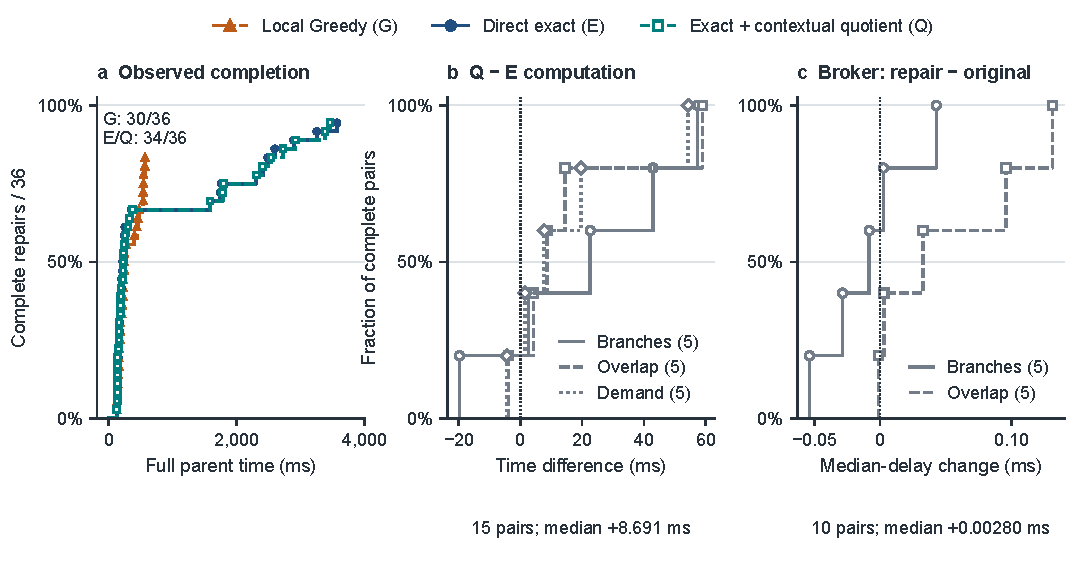
\includegraphics[width=\textwidth]{figures/03_complete_cost.pdf}
\caption{Historical complete cost: (a) repairs/all 36 specifications; (b) fifteen Q-minus-E parent-time pairs, five per condition; (c) ten Broker original/Q run-median delay pairs, five per condition. Missing pairs have no value; O has weaker safety guarantees.}\label{fig:cost}
\end{figure*}

\subsection{Effects of Edit Constraints and Rule Interactions}
Figure~\ref{fig:mechanisms} separates three input families. All assignments are generated/sorted, then rejected, checked or unvisited; early stopping saves checks only. E/Q counters coincide; G uses a different score counter.

Figure~\ref{fig:mechanisms} shows cap one infeasible and caps two/three sharing the same two-edit optimum. Inert atoms add search work without changing the optimum; overlap can require a neutral first edit that stalls G. E/Q counts coincide; slot options include unchanged/absent choices.



Historically, G completes 30/36 and E/Q 34/36; all four gains concern redundant Allows (G: six stalls; E/Q: one timeout/one infeasible each). Table~\ref{tab:gn1} separately compares all 36 existing specifications under cap three and five seconds/process, in one frozen random order; its 144 runs have separately recorded hardware and unisolated load.

With subscription \texttt{x/\#} and Allows \texttt{x/n0/\#} (priority 1), \texttt{x/n0/private/\#} (51), deleting the private Allow is neutral; direct private Deny collides; broad-Allow narrowing leaves private access. Exact repair uses neutral deletion then Deny at 52 (two operations, pattern cost five). $G_{N1}$ recovers all four gaps through neutral deletion then narrowing/Deny, matching E/Q completion and costs on 34 common returns. Its two stalls are not infeasibility proofs; new E/Q runs each time out twice. Single observations imply no speed advantage.

For completed policies (G $n=30$, E/Q $n=34$ each), shared median [min,max] summaries are operations $2\,[1,3]$, net rules $+2\,[-1,+3]$, pattern cost $10\,[0,15]$, changed originals $0\,[0,1]$ and additions $2\,[0,3]$; equal summaries do not mean matched repairs.

Nested $R_1\subseteq R_2\subseteq R_3$ add acknowledgement/administrative topics outside the forbidden subtree: all retain three rules/one operation. Four two-namespace cap/overlap cells are infeasible: one/two overlays need at least three/four edits, beyond caps one/two. Separately, size one succeeds at either cap; size two requires cap two and two edits. Artifacts retain exhaustive counts/nonzero times.



\subsection{Computational Cost and Scaling Behavior}
Figure~\ref{fig:cost}(a) combines completion and observed parent time $T_{mj}$ for outcome $s_{mj}$:
\[
 \widehat H_m(t)=\frac{1}{36}\sum_{j=1}^{36}
 \mathbf{1}[s_{mj}=\mathrm{complete},\ T_{mj}\le t].
\]
All 36 specifications remain in the denominator; failures never count as completion. These historical times are not budget sweeps.

For the fifteen complete Q/E pairs $\mathcal C$ (three conditions, five each; Figure~\ref{fig:cost}b),
\begin{equation}\label{eq:paired}
 \Delta_i=T_{Q,i}-T_{E,i},\quad
 \widetilde\Delta=\operatorname{median}_{i\in\mathcal C}\Delta_i.
\end{equation}
Q-minus-E differences have both signs; paired median is $+8.691$ ms, excluding five double-timeouts. Q retains all options: pressure scale medians [ranges] $21\,[18,25]$, $38\,[34,44]$, $54\,[50,65]$; completed timing representatives retain 29/36/38. No reduction/stable speed benefit appears.



Parent time includes startup, generation, preprocessing, enumeration/sorting, search, checking, I/O and cleanup. Pressure/timing provide 108/40 times and 106/30 RSS records; twelve timeouts (two/ten) lack RSS. Cleanup may exceed the five-second child budget; missing phases remain unknown. Marginal medians are not paired differences.

At scales one/two/three, E/Q complete 12/12, 12/12, 10/12; G completes 10/12 each. E/Q counters agree on 35/36 (one timeout lacks counts). Language settings are conditions, not repeats; host load limits timing inference.

\subsection{Broker Validation and Deployment Cost}
All 127 historical probes match independent predictions of loaded ACLs/defaults and identities. All 80 controls across forty snapshots arrive, without observed duplicates/publisher mismatch. Controls are separate from probes.

Priority-overlap snapshots use two topics per domain/property: O preserves required topics but blocks no forbidden ones; G/E/Q satisfy all four blocks, validating finite interpreter/export consistency.

Separately, two repaired snapshots yield 32 boundary probes: eight approved ordinary requests behave as predicted; eight unapproved ordinary and sixteen shared requests receive failure SUBACKs. Six wrong-credential/binding connections fail; four controls arrive. These counts do not extend the historical 127/80 or prove arbitrary shared-subscription security.

For ten original/Q pairs (branches/overlap, five each; Figure~\ref{fig:cost}c), let $d_r^m=\operatorname{median}_{j=1}^{10}\ell_{rj}^{m}$ and $\delta_r=d_r^Q-d_r^O$. Median $\delta_r$ is $+0.00280$ ms (six increases/four decreases). Branch median/p95 ranges are $[-0.0536,0.0428]$/$[-0.1309,0.0258]$ ms; overlap $[-0.0010,0.1311]$/$[0.0150,0.1950]$ ms. Thirty runs carry ten 64-byte QoS1 messages each: 300 nested observations. Unmatched originals are excluded; O has weaker safety. No microsecond-level superiority follows.

Configuration sizes and generation/readiness measurements remain in the artifact. Readiness includes process/plugin loading and polling; connection/subscription round trips are not isolated ACL costs, and host/observation effects remain unisolated.
Figure data/scripts, frozen-input identifiers and regression logs accompany the source artifact.
% END_SECTION evaluation

\FloatBarrier

% BEGIN_SECTION conclusion
\section{Conclusions and Future Work}
SPR-IoT combines explicit topic-language obligations, deployment-valid combination repair and independent execution checks. Finite-catalogue compliance is insufficient: repairs must preserve legitimate new branches while excluding forbidden descendants. Deployment-key constraints distinguish language-equivalent edits that cannot be substituted safely. One neutral bridge closes the strict greedy gap; contextual quotienting provides no observed candidate reduction or stable speed benefit. Broker checks confirm the tested static configurations; they establish neither unrestricted-client security nor generalization to independently sourced natural errors.

Future work will extend subscription and role composition, evaluate independent errors with documented requirements and compare systems under matched semantics. Unicode, shared subscriptions and session lifecycles require further language and deployment validation.
% END_SECTION conclusion

\bibliographystyle{IEEEtran}
\bibliography{references}
\end{document}
